%!TEX root=thesis.tex
\section{Surface Theory}

Investigating the properties of surfaces will form the basis on which our journey towards minimal surfaces rests. We will brave the perils that come in defining surfaces, and then use calculus on these surfaces to approximate the behavior at a point and extract information about the surface by extending on that approximation. Along the way we will make and derive various tools used for analyzing these surfaces, some of which we will bring along with us to Minimal Surfaces, others we will not, but they are interesting nonetheless and help illustrate some of the connections between Differential Geometry and various other branches of mathematics. We will look at parallels between these surfaces in $\RR^3$ and higher dimensional manifolds, though only briefly.

\subsection{Defining Surfaces in $\RR^3$}

% Simple surface
% TODO: Check to see if U needs to be connected.
% Refactored
Defining surfaces is not particularly difficult, but our methods require a set of considerations that can be subtle. We will first define a \emph{simple surface}, or coordinate patch, which represents a small open section of a larger surface. After considering that, we define a \emph{coordinate transformation}, a type of function whose presence between these patches implies some geometry-preserving properties. That done, we finally build up surfaces using an open covering of these coordinate patches, with the requirement that a coordinate transformation exist on their intersection. Along the way we will have plenty of examples to illustrate specific techniques and concepts introduced.

\begin{defn}
  Let $\sU$ be an open subset of $\RR^2$, then a function $\bx: \sU \to \RR^3$, written $\bx(u_1, u_2)$, is known as a \emph{simple surface} if it is injective and regular. The condition for regularity is that
  \[
    \frac{\partial\bx}{\partial u_1} \times \frac{\partial\bx}{\partial u_2} \neq 0
  \]
  across the domain of $\bx$. The function $\bx$ may also be referred to as a \emph{coordinate patch}.
\end{defn}

This definition is exactly what we want. Conceptually, the regularity of $\bx$ ensures that the mapping of $\sU$ to $\RR^3$ doesn't create any sharp creases or corners, but perhaps more relevant to our purposes, it also ensures that the partial derivatives form a linearly independent set. This will be critical later on.

% Monge Patch example
% TODO: Refactor and incorporate smooth/one-to-one
\begin{ex}
  Before going any further we introduce the \emph{monge patch}, a simple surface that will be instrumental as a simple example on which we can carry out our calculations. Let $f(x, y) = z$ be a function, then we can use this in the parameterization of our patch as follows: $\bx(u, v) = (u, v, f(u, v))$. Notice that
  \begin{align*}
    \frac{\partial\bx}{\partial u} \times \frac{\partial\bx}{\partial v} &= \left(-\frac{\partial f}{\partial u}, -\frac{\partial f}{\partial v}, 1\right)\\
    &\neq 0
  \end{align*}
  so it really is a simple surface.
\end{ex}

\begin{ex}
  % TODO: Fix akward wording
  Another fine example is the \emph{surface of revolution}. Given a curve in the $(r, z)$ with $r = r(t) > 0$ and $z = z(t)$, the surface of revolution generated by this curve (via rotation about the z-axis, is given by
  \[
    \bx(t, \theta) = (r(t)\cos\theta, r(t)\sin\theta, z(t)) \ .
  \]

  % NOTE: p15
  Assuming the curve is regular and injective, we can show that a surface of revolution really is a simply surface by simply checking. (A curve, say $\ba : (a, b) \to \RR^3$ is considered \emph{regular} when $\frac{d\ba}{dt} \neq 0$ for any $t$ in $(a, b)$.)

  A quick calculate yields the following:
  \begin{align*}
    \bx_1 &= (\dot{r}\cos{\theta}, \dot{r}\sin{\theta}, \dot{z})\\
    \bx_2 &= (-r(t)\sin{\theta}, r(t)\cos{\theta}, 0)\\
    \bx_1 \times \bx_2 &= (-\dot{z} r(t) \cos{\theta}, -\dot{z} r(t) \sin{\theta}, \dot{r}r(t))
  \end{align*}
  which is not $0$ since $r(t) > 0$, and then the original curve was regular so $\dot{r}, \dot{z} \neq 0$.
\end{ex}
% TODO: Example of an irregular surface


% NOTE: Coordinate Transformation Definition (p79)
\begin{defn}
  % TODO: Refactor
  Let $\sU, \sV$ be open subsets of $\RR^2$. A $C^k$ \emph{coordinate transformation} is an injective $C^k$ function $f: \sV \to \sU$ whose inverse $g:\sU \to \sV$ is also of class $C^k$. 
\end{defn}

In the propositions that follow we will see that the coordinate transformation preserves some of the geometric properties 

% TODO: Coordinate transformation information

Before getting to surfaces, we need to put an additional restriction on the coordinate patches that we build them with.

\begin{defn}
  Consider the inverse function for a coordinate patch $\bx$ from some subset $M$ of $\RR^3$ back to $\sU$, $\bx^{-1}: M \to \RR^2$ for some subset $M$ of $\RR^3$. We will say that this function is \emph{continuous} at a point $P$ if there is a neighborhood $U_P$ around the point such that $\bx^{-1}(U_P)\subset \sU$. The patch $\bx$ is considered \emph{proper} if $\bx^{-1}$ is continuous for all $P \in \bx(\sU)$.
\end{defn}

% NOTE: Surface definition (p89)
\begin{defn}
  A $C^k$ \emph{surface} in $\RR^3$ is a subset $M \subset \RR^3$ such that for every point $P \in M$ there is a proper $C^k$ coordinate patch whose image is in $M$ and which contains an $\eps$-neighborhood of $P$ for some $\eps > 0$. Furthermore, if both $\bx: \sU \to \RR^3$ and $\by: \sV \to \RR^3$ are such coordinate patches with $\sU^\prime = \bx(\sU), \sV^\prime = \by(\sV)$, then $y^{-1} \circ \bx: (x^{-1}(\sU^\prime \cap \sV^\prime)) \to (y^{-1}(\sU^\prime \cap \sV^\prime))$ is a $C^k$ coordinate transformation.
\end{defn}

% Picture here of the coordinate transformation requirement

% explanation of the coordinate transformation requirement.

% Example of a reason why this is necessary.

% Example of definition of the coordinate patches for a torus

One surface of revolution, the torus, has a patch given by the parameterization
\[
  \bx(u, v) = ((2 + \cos u)\cos v, (2 + \cos u) \sin v, \sin u)
\]
with the domain $\sU = \buildset{(u, v) \in \RR^2}{-\pi < u, v < \pi}$.

If we look at the diagram below we can see the areas not covered by this coordinate patch highlighted.
\begin{figure*}[t]
  \centering
  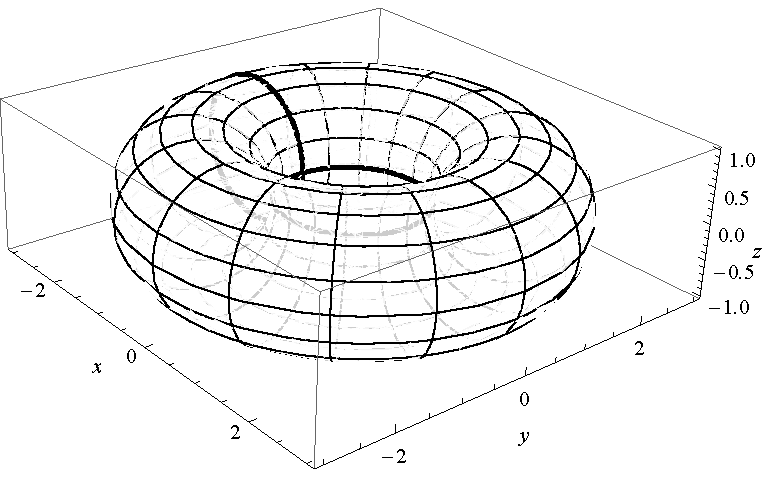
\includegraphics[width=0.5\textwidth]{figures/torus.pdf}
  \caption{Test}
\end{figure*}
In this case finding additional patches so the surface is covered is not difficult. We can use the same parameterization but with different bounds on the domain. If we let
\begin{align*}
  \sU_1 &= \buildset{(u, v) \in \RR^2}{-\pi < u < \pi, \frac{3\pi}{4} < v < \frac{5\pi}{4}}\\
  \sU_2 &= \buildset{(u, v) \in \RR^2}{-\pi < u < \pi, \frac{3\pi}{4} < v < \frac{5\pi}{4}}\\
  \sU_3 &= \buildset{(u, v) \in \RR^2}{-\pi < u < \pi, \frac{3\pi}{4} < v < \frac{5\pi}{4}}
\end{align*}
with the same parameterization for each, these will cover the outside of the torus on the negative $x$ side, the inside of the torus on the negative $x$ side, and the inside of the torus on the positive $x$ side, respectively.
% Check one of the intersections as a coordinate transformation

\subsection{Calculus on Surfaces}

% TODO: Explanation of title and the concepts that we will be introducing
\begin{defn}
  We consider two specific tangent vectors on a surface, the 
\end{defn}

\begin{unno_rem}
  We typically consider the partial derivative as the tangent vector of a curve holding one parameter of the function constant, so planting the base of the vector at the point at which it is evaluated.
\end{unno_rem}

% Continuity

% Properness

\begin{defn}
  The \emph{tangent plane} to a simple surface  $\bx: \sU \to \RR^3$ at the point $P = \bx(a, b)$ is the plane through $P$ perpendicular to $\bx_1(a, b) \times \bx_2(a, b)$. The \emph{unit normal} to the surface at $P$ is $\bn(a, b) = \frac{\bx_1 \times \bx_2}{\left|\bx_1 \times \bx_2\right|}$, where the right-hand side is evaluated at $(a, b)$. Note that $\bn(a, b)$ exists because $\bx_1 \times \bx_2 \neq 0$. It is perpendicular to the tangent plane at $P$.
\end{defn}

\begin{unno_rem}
  There are a few things to notice here. First, as $\bx_1$ and $\bx_2$ form a basis for the tangent plane and the unit normal is perpendicular to both, all together these three vectors form a basis for $\RR^3$. This will be useful later on as we consider the second derivative of curves at a point and will calculate them to put it into the context of the tangent plane.
\end{unno_rem}

\subsection{Tensors and Operators on Surfaces}

In this section we discover some of the tools that we will use to figure out the properties of surfaces in the next. Notice as we travel that the majority of these forms and tensors are really capturing very simple information, but we turn around and use them in combination to represent more complex or subtle properties of the surface. For this section assume that our operations are taking place on a simple surface and, while we will take some time to examine the fact that a property is indeed \emph{geometric} (i.e. independent of parameterization or the coordinate patch chosen for a point), where not shown or explicitly stated otherwise we will assume that the result is equivalent under a different parameterization. (For a more in-depth look at those specific considerations, see millman77)

% First fundamental form and metric tensor
\begin{unno_rem}
  One of the most fundamental operations in Euclidean space, allowing us notions of distance and angles between vectors, is the dot product (or more generally, the \emph{inner product}). We wish to have the same capability on our surface. Our definition is due to Millman77 and while we will see other representations later on, his is memorable. To motivate our construction, consider a surface $M \subset \RR^3$, $P$ a point on the surface, and two vectors $\bX$ and $\bY$ tangent to $M$ at $P$. Since $\bx_1$, $\bx_2$ form a basis for the tangent plane, in which $\bX$ and $\bY$ lie, we can write them as a linear combination and further, compute their inner product (denoted henceforth as $\la\phantom{x},\phantom{x}\ra$)
  \begin{align*}
    \bX &= \sum X^i\bx_i\\
    \bY &= \sum Y^j\bx_j\\
    \la\bX, \bY\ra &= \sum X^iY^j\la\bx_i, \bx_j\ra \ .
  \end{align*}
  With this in mind we make the following definition.
\end{unno_rem}

\begin{defn}
  The \emph{metric coefficients} are the functions defined by
  \[
    g_{ij}(u, v) = \la\bx_i(u, v), \bx_j(u, v)\ra \text{ or } g_{ij} = \la\bx_i, \bx_j\ra \ .
  \]
   % TODO: Expand here.
\end{defn}

% Second fundamental form

% Christoffel symbols

% Weingarten Map

\subsection{Curvature}

% Normal Curvature

% Geodesic curvature

% Geodesics


\subsection{Manifolds}